\graphicspath{{4_materials/figures/}}
\chapter{Materials}\label{chap:4}

\begin{quote}
  \textbf{Replication}\quad \emph{1.2}~The repetition of a scientific
  experiment or trial to obtain a consistent result.
\end{quote}

Such definition of \emph{replication} reveals the importance of reproducible
research, since confirmation of results obtained from independent studies is
considered the scientific gold standard to build our body of knowledge.

\citeauthor{peng2011reproducible} states the excitement and wanders that
computational science brings to the scientific landscape, but he also exposes
the limitations in the scientific community to evaluate its published findings
due to the lack of reproducibility. In order to overcome such limitations,
\citeauthor{peng2011reproducible} proposes reproducibility spectrum to be
covered in order to move from a mere non reproducible publication to fully
reproducible research (see \acs{fig}\,\ref{fig:reproducibility_spectrum}).
Specifically, \citeauthor{peng2011reproducible} argues that the original data,
the code of methods developed should both be made available along with the
executable that lead to the published results so that the three are fully
coupled\,\cite{peng2011reproducible}.

\begin{figure}
\centering
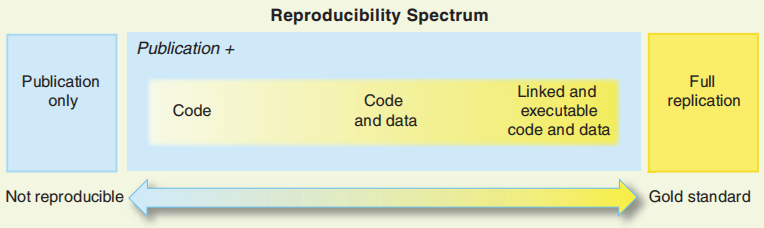
\includegraphics[width=.50\textwidth]{reproducibility_spectrum}
\caption[The spectrum of reproducibility.]{The spectrum of reproducibility (copyright by~\cite{peng2011reproducible}).}
\label{fig:reproducibility_spectrum}
\end{figure}

Furthermore, \citeauthor{varoquaux2015Software} in his article
%\citetitle{varoquaux2015Software}
\emph{Of Software and Science. Reproducible science: what, why, and how}
summarizes a discussion taken place in
\emph{\acs{mloss}} workshop regarding the issue of reproducible science. The
take away is that the reproducibility spectrum proposed by
\citeauthor{peng2011reproducible} falls short because it focuses on providing material to
backup publications but oversights the importance of sound reusable material and
methods, which are the foundation of future scientific developments despite
being cast out of the success formula in academia where only impact factor seems
to matter.

With all this\footnote{better connector needed. Maybe a sentece}, the structure
of this chapter is going to appear odd to some readers since our intention with
this \nameref{chap:4} chapter is two fold:
(i) use this chapter to position ourselves with respect of reproductible
research;
and, (ii) describe all the resources or outcomes from this thesis that make for
reproductible research.

The former part is more of philosophical discussion or proclamation of the
working systems and protocols emerging from this thesis work. While the later is
a more concrete description of the resources to reproduce the work of our
thesis. Underlying design choices are out of the scope of this chapter. Those
regarding the methodologies developed for this thesis work can be found in other chapters.

\section{Our efforts towards reproducible research.}
To conduct our research we have developed working strategies based on existing
and in-house platforms. This section describes its current status with upcoming
fixtures resulting from writing and reviewing this thesis, since these working
strategies follow an iterative incremental procedure.

\subsection{\acs{iccvb}}
For this purpose we have created the \acs{iccvb} website and its associated
github community, which stands on the following core pillars stated on the website:

\paragraph{Why?. our vision: to democratize the access to research}
The first need in modern research, regardless its application domain, is related to the access to reliable data for its subsequent study.

However, data gathering is an entrance barrier for most of the researchers mainly due to factors as diverse costs, infrastructure, availability, etc. Moreover, isolated endeavours to gather these data without granting public access lead to the creation of muda ("waste"): waste of resources and inability to compare results and validate conclusions.

Despite being highlighted by numerous research works, the lack of usable, public, reliable, and accessible data remains disregarded in many fields. The I2CVB is a wake-up call for addressing and breaking the entrance barriers in research due to data and/or isolation by applying collaborative strategies.

\paragraph{What?. mission: to democratize the access to research}
The lack of common data combined with non-aggregated assessing strategies result in non-existent or misleading comparisons make difficult to acknowledge relevant novel methodologies. A common duty to the research and development communities is to overcome these limitations, which can be successfully addressed by co-creation and collaborative work.

I2CVB aims at serving as foundation for collecting and sharing data as well as providing common evaluation methodologies. Furthermore, the use of common data and evaluation is the only way to achieve fair comparison.

\paragraph{Who?. protagonists: Research groups and individuals from all walks of life to shape a transparent community}
I2CVB creates for everyone the opportunity to pursue common goals through sharing, collaborating and team-working, to empower the individuals by taking advantages of personal skills and resources. As a consequence, young researchers will find an eco-system for self-improvement in which work will be rewarded through benchmarking compilation.

\paragraph{How?. strategy Transfer successful practises from Free Software and Quality Managemen}
I2CVB community challenges the impossible as well as the current status quo in research. Therefore, we strive to settle a multi-skilled community pursuing common goals to achieve excellence through collaborative continuous improvement.

At I2CVB, we believe that Free Software and Quality Management have already reshaped the world and that it is time to apply some of the successful practices learned in such domains to expand the boundaries of research in computer vision and specially for the medical imaging case.

\subsection{Software Quality}

All the different source code implemented for this thesis have been released to support future development and the possibility to build a consistent benchmark.
All available code is primarily developed in Python with a concern of:
(i) \emph{Quality insurance} by developing unit tests, automatic code quality checking, and code consistency checking using \texttt{PEP8} standards;
(ii) \emph{Continuous integration} is achieved through tools as Travis CI to easily integrate new contributions and ensure back-compatibility;
(iii) \emph{Community-based development} by using collaborative tools --- git, GitHub, and gitter --- to ease collaborative programming, issue tracking, code integration, and idea discussions;
(iv) \emph{Documentation} through a description of the developed API.

\subsection{Working strategy}
As aforesaid, we developed a website and a github community. The website is used
mainly as facade to our project but its core is the \acs{iccvb} github community
and this is how we strive for repeatable research.

Our research is based on collecting data, coding experiments, interpret and
communicate the observations. Back to the data, re-code the experiments,
re-interpret the observations. In essence research is an iterative incremental
process that require to ensure the quality at each step and its final deliver of
each iteration is a manuscript that pin-point a position in the history of this
research. For some publication it might refer to an small portion of our research
or quick proof of concept while for other works it refers to a larger portion.

Consolidating an analysis pipeline, a standard visualization, or any
computational aspect of work into a software library is a sure way to make
the publications more reproducible. Maintaining the library will ensure that results
are still reproducible on new hardware, or with evolution of the general
software stack. Documentation and curated examples will lower the bar to reuse
and facilitate replication of the original scientific results.
To avoid feature technical debt, libraries call for focused efforts
on selecting the most important operations and become projects on their own.\,\cite{varoquaux2015Software}.

\paragraph{publication releases}
The rest of this section summarizes our working strategy based on the experience
acquired during this thesis that lead to the aforesaid. Publications,
experiments, etc. become projects. These projects have their code and
documentation hosted in github while its associated publications are subprojects
with their source also hosted in github. This allow us to review projects and
publications in the same manner taking advantage of issue tracking and \acs{ci}.
The data of the project is hosted at \acs{cern}, provided with a \acs{doi} using
\emph{Zenodo} and disseminated through \acs{iccvb} website. At the time of
publication, the code is released to freeze its state. \emph{Zenodo} provides a
\acs{doi} to reference the release. Releases are incorporated to the \acs{ci}
systems to detect back-compatibility breaks and fix them by release reviews.
Evolution of our tools and libraries also captured by the \acs{ci}.

\section{Prostate data}
This section describe the datasets used in this thesis which are also available
through the \acs{iccvb} website.

\subsection{\SI{1.5}{\tesla} General Electric scanner}

The \ac{mpmri} data are acquired from a cohort of patients with higher-than-normal level of \ac{psa}.
The acquisition is performed using a \SI{1.5}{\tesla} whole body GE Signa \ac{mri} scanner (General Electric, Milwaukee, WI, USA) with an endorectal coil (Medrad, Pittsburgh, PA, USA), using sequences to obtain \ac{t2w}-\ac{mri}, \ac{dce}-\ac{mri}, \ac{dw}-\ac{mri}, and \ac{mrsi}.
Aside of the \ac{mri} examination, these patients also have undergone a guided-biopsy.
% The dataset is composed of a total of 20 patients of which 18 patients have biopsy proven \ac{cap} and 2 patients are ``healthy'' with negative biopsies.
% Therefore, 13 patients have a \ac{cap} in the \ac{pz}, 3 patients have \ac{cap} in the \ac{cg}, 2 patients have invasive \ac{cap} in both \ac{pz} and \ac{cg}, and finally 2 patients are considered as ``healthy''.
% An experienced radiologist has segmented the prostate organ as well as the prostate zones, and \ac{cap} on the \ac{t2w}-\ac{mri}.

Three-dimensional \ac{t2w} fast spin-echo (\ac{tr}/\ac{te}/\ac{etl}: \SI{3480}{\ms}/\SI{113.6}{\ms}/16, slice thickness: \SI{3}{\mm}) images are then acquired in an oblique axial plane with a  $320 \times 224$ acquisition matrix and a pixel spacing of \SI{0.27}{\milli\metre}.

%The nominal matrix and \ac{fov} of the 3D \ac{t2w} fast spin-echo images are \SI[product-units=repeat]{320x256}{\milli\metre\squared} and \SI[product-units=repeat]{280x240}{\milli\metre\squared}, respectively, thereby affording sub-millimetric pixel resolution within the imaging plane.

\ac{dce}-\ac{mri} is performed using a fat suppressed 3D fast spoiled gradient echo (\ac{tr}/\ac{te}/Flip angle: \SI{4.42}{\ms}/\SI{2.10}{\ms}/\SI{12}{\degree}; Matrix: $320 \times 192$; slab of 40 partitions of \SI{3.5}{\mm} thickness; temporal resolution: \SI{10}{\s}/slab over approximately \SI{5}{\minute}).
A power injector (Medrad, Indianola, USA) is used to provide a bolus injection of Gd-DTPA (Dotarem, Guerbet, Roissy, France) at a dose of \SI{0.2}{\ml} Gd-DTPA/kg of body weight.

\ac{dw}-\ac{mri} images have been acquired using the single-shot spin-echo echo-planar imaging (EPI) technique.
The diffusion-encoding gradients have been applied using a pulsed gradient spin-echo technique resulting in diffusion images acquired at 2 b-values --- i.e., \SI{100}{\second\per\milli\meter\squared} and \SI{1400}{\second\per\milli\meter\squared} --- and in the 3 orthogonal directions.
Sequential sampling of the k-space has been used with a \ac{te} of \SI{100.1}{\ms}, a \ac{tr} of \SI{10825}{\ms}, a bandwidth of \SI{1953}{\hertz\per\px}, and an acquisition matrix size of $128 \times 128$.

\ac{mrsi} is performed using a water and lipid suppressed double-spin-echo point-resolved spectroscopic (PRESS) sequence optimized for quantification detection of choline and citrate metabolites.
Water and lipid have been suppressed using a dual-band spectral spatial pulse technique.
%In order to eliminate signals from adjacent tissues, especially periprostatic lipids and the rectal wall up to 8 outer voxel saturation pulses have been used.
Datasets have been acquired as $16 \times 8 \times 8$ phase-encoded spectral arrays, a \ac{te} of \SI{130}{\ms}, a \ac{tr} of \SI{1000}{\ms}.%, and \SI{13}{\minute} of acquisition time.
%A spectral bandwidth of \SI{1250}{\hertz} has been used with 512 data points.
%A combination of an elliptic weighted averaged k-space acquisition scheme 3D filtering of the signal in k-space have been used, the latter in order to reduce intervoxel signal combination.
%Shimming has been carried out using the Siemenbens 3D Mapshim routine on a voxel adapted to the volume of the entire prostate gland.

\subsection{\SI{3}{\tesla} Siemens scanner}

The \ac{mpmri} data are acquired from a cohort of patients with higher-than-normal level of \ac{psa}.
The acquisition is performed using a \SI{3}{\tesla} whole body \ac{mri} scanner (Siemens Magnetom Trio TIM, Erlangen, Germany) using sequences to obtain \ac{t2w}-\ac{mri}, \ac{dce}-\ac{mri}, \ac{dw}-\ac{mri}, and \ac{mrsi}.
Aside of the \ac{mri} examination, these patients also have undergone a guided-biopsy.
The dataset is composed of a total of 20 patients of which 18 patients have biopsy proven \ac{cap} and 2 patients are ``healthy'' with negative biopsies.
Therefore, 13 patients have a \ac{cap} in the \ac{pz}, 3 patients have \ac{cap} in the \ac{cg}, 2 patients have invasive \ac{cap} in both \ac{pz} and \ac{cg}, and finally 2 patients are considered as ``healthy''.
An experienced radiologist has segmented the prostate organ --- on \ac{t2w}-\ac{mri}, \ac{dce}-\ac{mri}, and \ac{adc}-\ac{mri} --- as well as the prostate zones --- i.e., \ac{pz} and \ac{cg} ---, and \ac{cap} on the \ac{t2w}-\ac{mri}.

A \SI{3}{\mm} slice fat-suppressed \ac{t2w} fast spin-echo sequence (\ac{tr}/\ac{te}/\ac{etl}: \SI{3400}{\ms}/\SI{85}{\ms}/13) is used to acquire images in sagittal and oblique coronal planes, the latter planes being orientated perpendicular or parallel to the prostate \ac{pz} – rectal wall axis.
Three-dimensional \ac{t2w} fast spin-echo (\ac{tr}/\ac{te}/\ac{etl}: \SI{3600}{\ms}/\SI{143}{\ms}/109, slice thickness: \SI{1.25}{\mm}) images are then acquired in an oblique axial plane.
The nominal matrix and \ac{fov} of the 3D \ac{t2w} fast spin-echo images are \SI[product-units=repeat]{320x256}{\milli\metre\squared} and \SI[product-units=repeat]{280x240}{\milli\metre\squared}, respectively, thereby affording sub-millimetric pixel resolution within the imaging plane.

\ac{dce}-\ac{mri} is performed using a fat suppressed 3D T$_1$ VIBE sequence (\ac{tr}/\ac{te}/Flip angle: \SI{3.25}{\ms}/\SI{1.12}{\ms}/\SI{10}{\degree}; Matrix: $256 \times 192$; \ac{fov}: $280 \times 210$ (with \SI{75}{\percent} rectangular \ac{fov}); slab of 16 partitions of \SI{3.5}{\mm} thickness; temporal resolution: \SI{6}{\s}/slab over approximately \SI{5}{\minute}).
A power injector (Medrad, Indianola, USA) is used to provide a bolus injection of Gd-DTPA (Dotarem, Guerbet, Roissy, France) at a dose of \SI{0.2}{\ml} Gd-DTPA/kg of body weight.

\ac{dw}-\ac{mri} images have been acquired using the single-shot spin-echo echo-planar imaging (EPI) technique.
As proposed by \citeauthor{stejskal1965spin}~\cite{stejskal1965spin}, the diffusion-encoding gradients have been applied using a pulsed gradient spin-echo technique resulting in diffusion images acquired at 2 b-values --- i.e., \SI{100}{\second\per\milli\meter\squared} and \SI{800}{\second\per\milli\meter\squared} --- and in the 3 orthogonal directions.
Sequential sampling of the k-space has been used with a \ac{te} of \SI{101}{\ms}, a \ac{tr} of \SI{4200}{\ms}, and a bandwidth of \SI{1180}{\hertz\per\px}.
Other parameters included a \ac{fov} of \SI{240}{\milli\metre}, an acquisition matrix size of $128 \times 128$ and a slice thickness of \SI{3.5}{\milli\metre}.
The \ac{adc} map has been directly generated by the Siemens workstation from the raw data on a pixel-by-pixel basis.

\ac{mrsi} is performed using a water and lipid suppressed double-spin-echo point-resolved spectroscopic (PRESS) sequence optimized for quantification detection of choline and citrate metabolites.
Water and lipid have been suppressed using a dual-band spectral spatial pulse technique.
In order to eliminate signals from adjacent tissues, especially periprostatic lipids and the rectal wall up to 8 outer voxel saturation pulses have been used.
Datasets have been acquired as $16 \times 12 \times 16$ --- interpolated to $16 \times 16 \times 16$ phase-encoded spectral arrays, a \ac{te} of \SI{140}{\ms}, a \ac{tr} of \SI{720}{\ms} and \SI{13}{\minute} of acquisition time.
A spectral bandwidth of \SI{1250}{\hertz} has been used with 512 data points.
A combination of an elliptic weighted averaged k-space acquisition scheme 3D filtering of the signal in k-space have been used, the latter in order to reduce intervoxel signal combination.
Shimming has been carried out using the Siemenbens 3D Mapshim routine on a voxel adapted to the volume of the entire prostate gland.
Additional unsuppressed water acquisitions at \ac{te} of \SI{30}{\ms}, \SI{80}{\ms}, and \SI{140}{\ms} of \SI{1.5}{\minute} have also been performed in order to allow quantification with respect to prostate water.
Systematic verification of the global shim --- i.e., over the complete 3D PRESS-selected volume --- revealed line widths at half-height of the water peak of the order of \SIrange{20}{30}{\hertz}, routinely.
The line widths for individual voxels are of the order of \SIrange{8}{12}{\hertz}.
The total examination time, including the time spent positioning the patient, is approximately 45 minutes.


\section{\texttt{imbalanced-learn} toolbox}\label{chp4:sec:imblearn}

The \texttt{imbalanced-learn} toolbox is an open-source python toolbox aiming at providing a wide range of methods to cope with the problem of imbalanced dataset frequently encountered in machine learning and pattern recognition.
The implemented state-of-the-art methods can be categorized into 4 groups: (i) under-sampling, (ii) over-sampling, (iii) combination of over- and under-sampling, and (iv) ensemble learning methods.
The proposed toolbox only depends on \texttt{numpy}, \texttt{scipy}, and \texttt{scikit-learn} and is distributed under MIT license.
Furthermore, it is fully compatible with \texttt{scikit-learn} and is part of the \texttt{scikit-learn-contrib} supported project.
Documentation, unit tests as well as integration tests are provided to ease usage and contribution.
The toolbox is publicly available in GitHub\footnote{\url{https://github.com/scikit-learn-contrib/imbalanced-learn}}.

To illustrate the developed API and the compatibility with \texttt{scikit-learn}, an example of a pipeline using a \ac{pca} decomposition, a \ac{smote} over-sampler, and a \ac{knn} classifier is presented below:

\begin{lstlisting}[language=Python, caption=Code snippet to over-sample a dataset using \acs*{smote} in conjunction with \ac{pca} and a \ac{knn} classifer.]
from sklearn.datasets import make_classification
from sklearn.cross_validation import train_test_split as tts
from sklearn.decomposition import PCA
from sklearn.neighbors import KNeighborsClassifier as KNN
from sklearn.metrics import classification_report
from imblearn.over_sampling import SMOTE
from imblearn.pipeline import Pipeline
X, y = make_classification(n_classes=2, class_sep=2,
                           n_informative=3, n_redundant=1, flip_y=0,
                           n_features=20, n_clusters_per_class=1,
                           n_samples=1000, weights=[0.1, 0.9])
pca = PCA()
smt = SMOTE()
knn = KNN()
pipeline = Pipeline([('smt', smt), ('pca', pca), ('knn', knn)])
X_train, X_test, y_train, y_test = tts(X, y, random_state=42)
pipeline.fit(X_train, y_train)
y_hat = pipeline.predict(X_test)
\end{lstlisting}

\section{\texttt{protoclass} toolbox}\label{chp4:sec:protoclass}

The \texttt{protoclass} toolbox is an open-source python toolbox providing tools for fast prototyping of machine learning pipeline in medical imaging.
It implements most of the state-of-the-art feature detection techniques presented in \acs{chp}\,\ref{chap:3}.
To illustrate the API, an example is given in which a \ac{t2w}-\ac{mri} volume is normalized and the voxels corresponding to the prostate are extracted and can be used easily with \texttt{scikit-learn}.

\begin{lstlisting}[language=Python, caption=Code snippet to normalize a volume and extract some voxels.]
import os
from protoclass.data_management import T2WModality
from protoclass.data_management import GTModality
from protoclass.preprocessing import GaussianNormalization
from protoclass.extraction import IntensitySignalExtraction

# Define the path the different data path
path_t2w = '/data/T2W'
path_gt = ['/data/GT/prostate']
label_gt = ['prostate']

# Read the T2W
t2w_mod = T2WModality()
t2w_mod.read_data_from_path(path_t2w)

# Read the ground-truth
gt_mod = GTModality()
gt_mod.read_data_from_path(label_gt, path_gt)

# Normalize the T2W modality
t2w_norm = GaussianNormalization(T2WModality())
t2w_norm.fit(t2w_mod, ground_truth=gt_mod, cat=label_gt[0])
t2w_mod = t2w_norm.normalize(t2w_mod, ground_truth=gt_mod,
                             cat=label_gt[0])

# Extract the voxel from the prostate
ise = IntensitySignalExtraction(t2w_mod)
data = ise.transform(t2w_mod, ground_truth=gt_mod, cat=label_gt[0])
\end{lstlisting}

